\section{Results and logs}
\label{sec:Results_and_Logs}

\subsection{Results}
When executing a user application we consider different type of results:
\begin{itemize}
 \item \textbf{Application Output:} Output generated by the application.
 \item \textbf{Application Files:}  Files used or generated by the application.
 \item \textbf{Tasks Output:} Output generated by the tasks invoked from the application.
\end{itemize}

Regarding the application output, COMPSs will preserve the application output but will add some pre and post output to indicate
the COMPSs Runtime state. Figure \ref{fig:compss_out} shows the standard output generated by the execution of the 
simple java application. The green box highlights the application \textit{stdout} while the rest of the output is produced by COMPSs.  
\begin{figure}[h!]
  \centering
    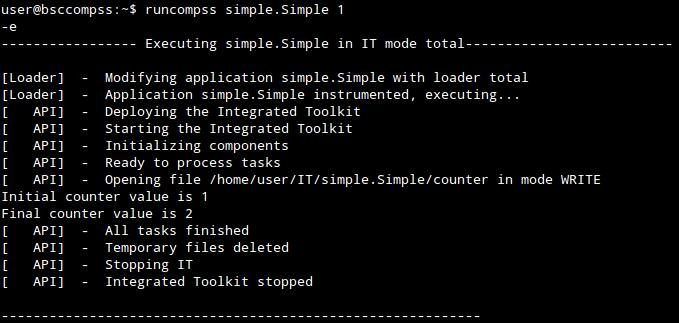
\includegraphics[width=0.6\textwidth]{./Sections/3_Results_and_Logs/Figures/simple_java_stdout.jpeg}
    \caption{Ouput generated by the execution of the \textit{Simple} java application with COMPSs}
\end{figure}
\label{fig:compss_out}

Regarding the application files, COMPSs \textbf{does not modify} any of them and thus, the
results obtained by executing the application with COMPSs are the same than the ones generated by the sequential execution
of the application.

Regarding the task output, COMPSs does introduce some modifications due to the fact that tasks can be executed in remote
machines. Considering that we call a job the execution of a task in a given resource, after the execution, COMPSs stores 
the \textit{stdout} and the \textit{stderr} of each job inside the \textbf{$/home/\$USER/.COMPSs/\$APPNAME/\$EXEC\_$
$NUMBER/jobs/$}
directory.

Figure \ref{fig:hello_exec_results} shows an example of the results obtained from the execution of the \textit{Hello} java 
application. At rigth we provide the sequential execution of the application and, at left, its equivalent COMPSs execution. 
Notice that, the sequential execution produces the \" Hello World!\" message in the \textit{stdout} while the COMPSs execution 
stores the message inside the \textit{$job1\_NEW.out$} file.
\begin{figure}[h!]
  \centering
    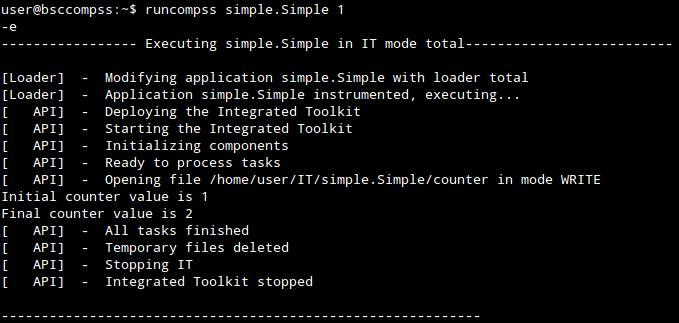
\includegraphics[width=0.6\textwidth]{./Sections/3_Results_and_Logs/Figures/hello_seq_stdout.jpeg}
    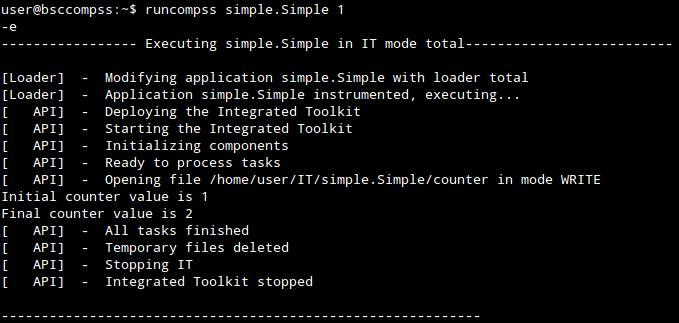
\includegraphics[width=0.6\textwidth]{./Sections/3_Results_and_Logs/Figures/hello_compss_stdout_and_job.jpeg}
    \caption{Result comparison between a sequential and a COMPSs execution of the \textit{Hello} java application}
    \label{fig:hello_exec_results}
\end{figure}

\newpage

\subsection{Logs}
COMPSs includes three log levels for running applications but users can modify them or add more levels by editing the
logger files under the \textit{/opt/COMPSs/Runtime/configuration/log/} folder. Any of these log levels can be selected by 
adding the \textit{$--log\_level=<debug | info | off >$} flag to the runcompss command. The default value is \textit{off}.

The logs generated by the execution number $NUM\_EXEC$ of the application APP by the user USER are stored under
\textit{$/home/\$USER/.COMPSs/\$APP/\$NUM\_EXEC/$} folder (from this point on: \textbf{base log folder}). The execution number is 
automatically tracked to prevent the loss of data from previous executions, but users do not need to take care of this value. 

When running COMPSs with \textbf{log level off} only the errors are reported. This means that the \textit{base log folder} will be
empty if no error has occured. If somehow the application failed, a \textit{jobs} folder will appear containing the \textit{stdout}
and the \textit{stderr} of each failed job. Figure \ref{listing:logs_off} shows the logs generated by the execution of the simple 
java application (without errors) in \textbf{off} mode. 
\begin{lstlisting}[language=bash]
compss@bsc:~$ ls -l ~/.COMPSs/simple.Simple_01/
\end{lstlisting}
\label{listing:logs_off}

When running COMPSs with \textbf{log level info} the \textit{base log folder} will contain two files (\textbf{runtime.log} and 
\textbf{resources.log}) and one folder (\textit{jobs}). The \textbf{runtime.log} file contains the execution information retrieved 
from the master resource; including the file transfers and the job submission details. The \textbf{resources.log} file contains 
information about the available resources such as the number of processors of each resource (slots), the information about running or 
pending tasks in the resource queue and the created and destroyed resources. The \textit{jobs} folder contains two files 
per submitted job; one for the \textit{stdout} and another for the \textit{stderr}. As an example, Figure \ref{listing:logs_info} 
shows the logs generated by the same execution than the previous case but with \textbf{info} mode. 
\begin{lstlisting}[language=bash]
compss@bsc:~$ tree ~/.COMPSs/simple.Simple_01/
\end{lstlisting}
\label{listing:logs_info}

The runtime.log and resources.log are quite large files and, thus, should be only checked by advanced users. For an
easier interpretation of these files the COMPSs Framework includes a monitor tool. For further information about the COMPSs Monitor
please check Section \ref{subsec:monitor}.

Figures \ref{fig:simple_runtimelog} and \ref{fig:simple_resourceslog} provide the content of these two files generated
by the execution of the \textit{Simple} java application. 
\begin{figure}[h!]
  \centering
    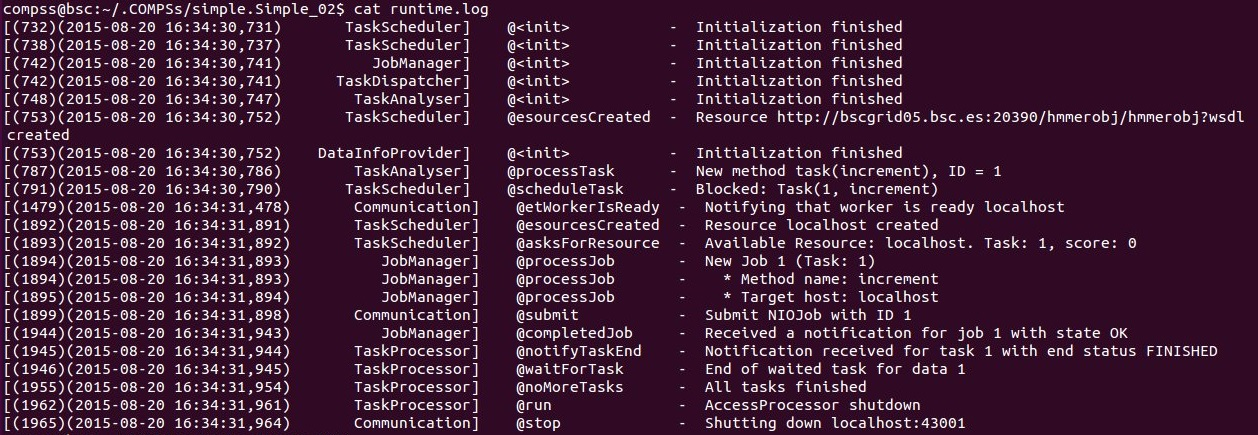
\includegraphics[width=0.95\textwidth]{./Sections/3_Running_Apps/Figures/simple_runtimelog.jpeg}
    \caption{runtime.log generated by the execution of the \textit{Simple} java application}
\end{figure}
\label{fig:simple_runtimelog}

\begin{figure}[h!]
  \centering
    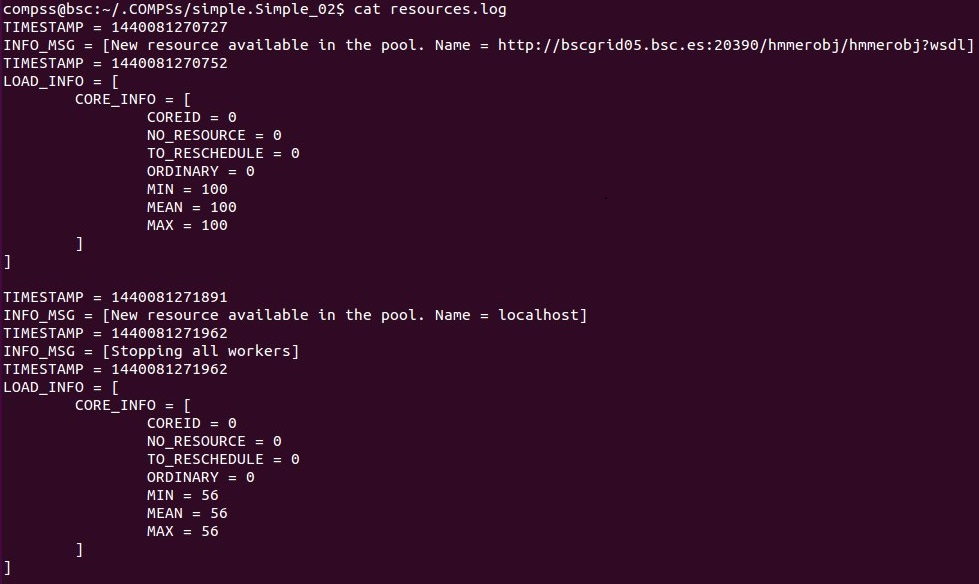
\includegraphics[width=0.95\textwidth]{./Sections/3_Running_Apps/Figures/simple_resourceslog.jpeg}
    \caption{resources.log generated by the execution of the \textit{Simple} java application}
\end{figure}
\label{fig:simple_resourceslog}

Running COMPSs with \textbf{log level debug} generates the same files as the info log level but with more detailed information.
Moreover, the COMPSs Runtime state is printed out on the \textit{stdout}. The runtime.log and the resources.log
files generated in this mode can be \textbf{extremely large}. Consequently, the users should take care of their quota and manually
erase these files if needed. \newline

Furthermore, when running other runcompss flags (such as monitoring or tracing) additional folders will appear inside the 
\textit{base log folder}. The meaning of the files inside these folders is explained in Section \ref{sec:Tools}. 
